%
% Selección de comparación de desempeño.
% Implementación de programa tokenizador, reporte técnico.
%
% Proyecto Lovelace.
%

\subsection{Comparación de desempeño}
\label{sec:comparacion}

Como se indicó en la introducción de este trabajo, la tokenización digital es un
proceso relativamente nuevo y la mayoría de los proveedores de este servicio
aprovechan la confusión y desinformación existente para atraer a clientes
potenciales, pues pocos comparten la manera en que crean sus \glspl{gl:token}.
Esta sección busca resarcir un poco el daño, presentado una comparación entre
los tiempos de respuesta de tokenización y detokenización de los algoritmos
implementados.

En la tabla~\ref{tabla:tiempos_tokenizacion} se puede observar el tiempo
promedio que le toma a cada algoritmo hacer una operación de tokenización
y detokenización; estos valores se obtuvieron al ejecutar varias veces 15K
operaciones de tokenización y detokenización, luego obtener el promedio
y, finalmente, dividir entre 15K. Los algoritmos están divididos en reversibles
y no reversibles, pues, dadas sus características, no sería muy parejo
compararlos entre sí; por ejemplo, basta hacer una consulta en la base de datos
para hacer la detokenización en los algoritmos irreversibles; mientras que en
los reversibles hay que hacer el proceso inverso, o uno equivalente, para
poder obtener de nuevo el \gls{gl:pan}.

\begin{table}
  \begin{center}
    \begin{tabular}{c|c|c|}
      \cline{2-3}
      & Tokenización & Detokenización \\
      \hline
      \multicolumn{1}{|c|}{BPS}
        & 359.088   $\mu$s & 357.620 $\mu$s   \\\hline
      \multicolumn{1}{|c|}{FFX}
        & 274.905   $\mu$s & 275.147 $\mu$s   \\\hline

      \multicolumn{1}{|c|}{TKR}
        & 74.424  $m$s & 669.203 $\mu$s   \\\hline
      \multicolumn{1}{|c|}{AHR}
        & 70.041  $m$s & 719.729 $\mu$s   \\\hline
      \multicolumn{1}{|c|}{DRBG}
        & 75.247  $m$s & 696.643 $\mu$s  \\\hline
    \end{tabular}

    \caption{Comparación de tiempos de tokenización.}
    \label{tabla:tiempos_tokenizacion}
  \end{center}
\end{table}

Los datos de la tabla~\ref{tabla:tiempos_tokenizacion} fueron utilizados para
crear una serie de gráficas: en la figura~\ref{figura:tok_todos} se comparan los
tiempos de tokenización y detokenización de todos los algoritmos, tanto
reversibles como irreversibles; la velocidad de los algoritmos reversibles es
notoria, en especial al momento de la operación de tokenización. Posteriormente,
en la figura~\ref{figura:tok_rev}, se compararon solo los algoritmos reversibles
(\hyperref[sec:bps]{BPS} y \hyperref[sec:ffx]{FFX}), siendo el segundo el más
rápido de los dos; la similitud del comportamiento de estos algoritmos en ambas
operaciones se debe a que se realizan casi las mismas operaciones para cifrar
como para cifrar. Finalmente, se compararon los tiempos para los algoritmos
irreversibles en las gráficas de la figura~\ref{figura:tok_irrev}: durante las
operaciones de tokenización, aunque están relativamente cerrados los tiempos,
\hyperref[sec:ahr]{AHR} queda como el más rápido de los tres, mientras que
\hyperref[sec:drbg_lista]{DRBG} queda en segundo lugar; es menester recordar
porqué estos algoritmos toman más tiempo: \hyperref[sec:ahr]{AHR} utiliza
\gls{gl:cifrado_caminata_ciclica}, y, al generar un \gls{gl:token}, consulta la
base de datos, pues permite tener más de un \gls{gl:token} por \gls{gl:pan};
además, tanto \hyperref[sec:tkr]{TKR2} como \hyperref[sec:drbg_lista]{DRBG}
necesitan bits pseudoaleatorios, y si el generador de bits pseudoaleatorios
tarda en obtenerlos, los algoritmos se ven afectados; finalmente, en las
operaciones de detokenización, \hyperref[sec:drbg_lista]{DRBG} es el más rápido
de todos, mientras que \hyperref[sec:ahr]{AHR} queda como el más lento de los
tres. En la figura~\ref{figura:tok_comp} se puede ver la diferencia de tiempos
entre las operaciones de tokenización y detokenización; los tiempos de los
algoritmos reversibles son casi idénticos en ambas operaciones, mientras que
se observa un cambio notorio entre los tiempos de tokenización y detokenización
de los irreversibles.

\begin{figure}
  \centering
  \begin{subfigure}{1\textwidth}
    \begin{center}
      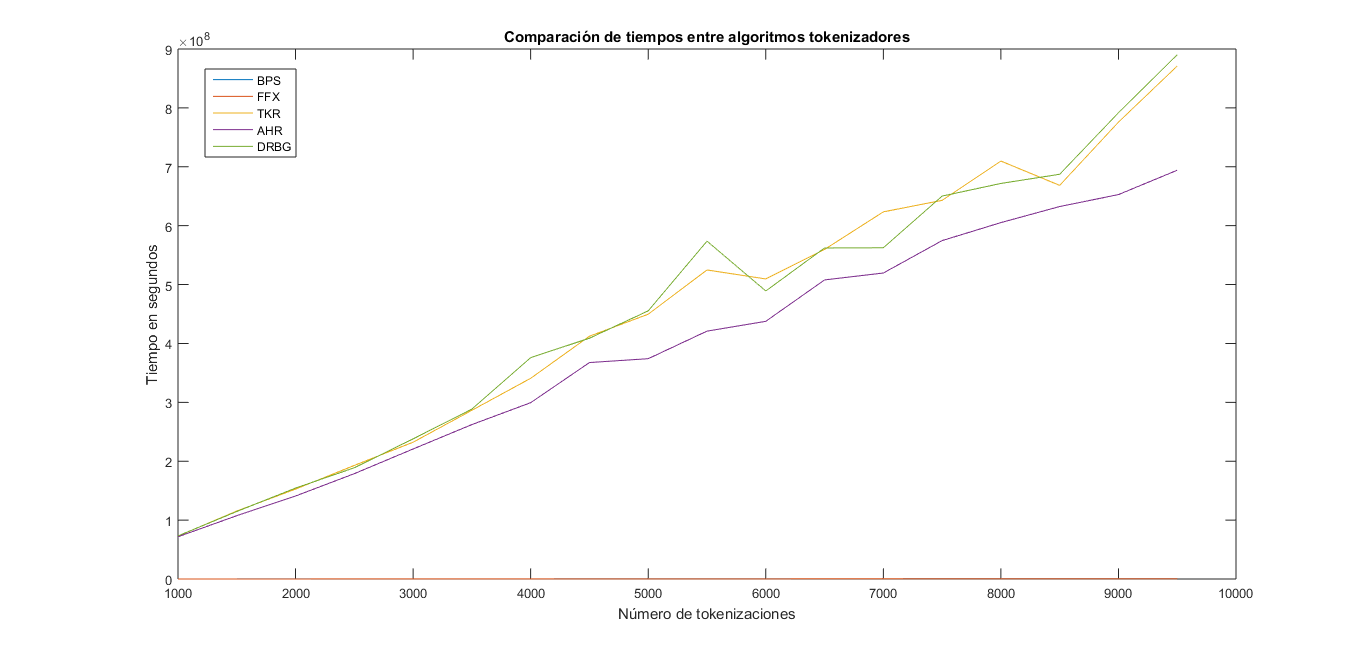
\includegraphics[width=1\linewidth]
        {../../../../../diagramas_comunes/desempenio/tok_todos}
      \caption{Tiempos de tokenización.}
    \end{center}
  \end{subfigure}
  \begin{subfigure}{0.9\textwidth}
    \begin{center}
      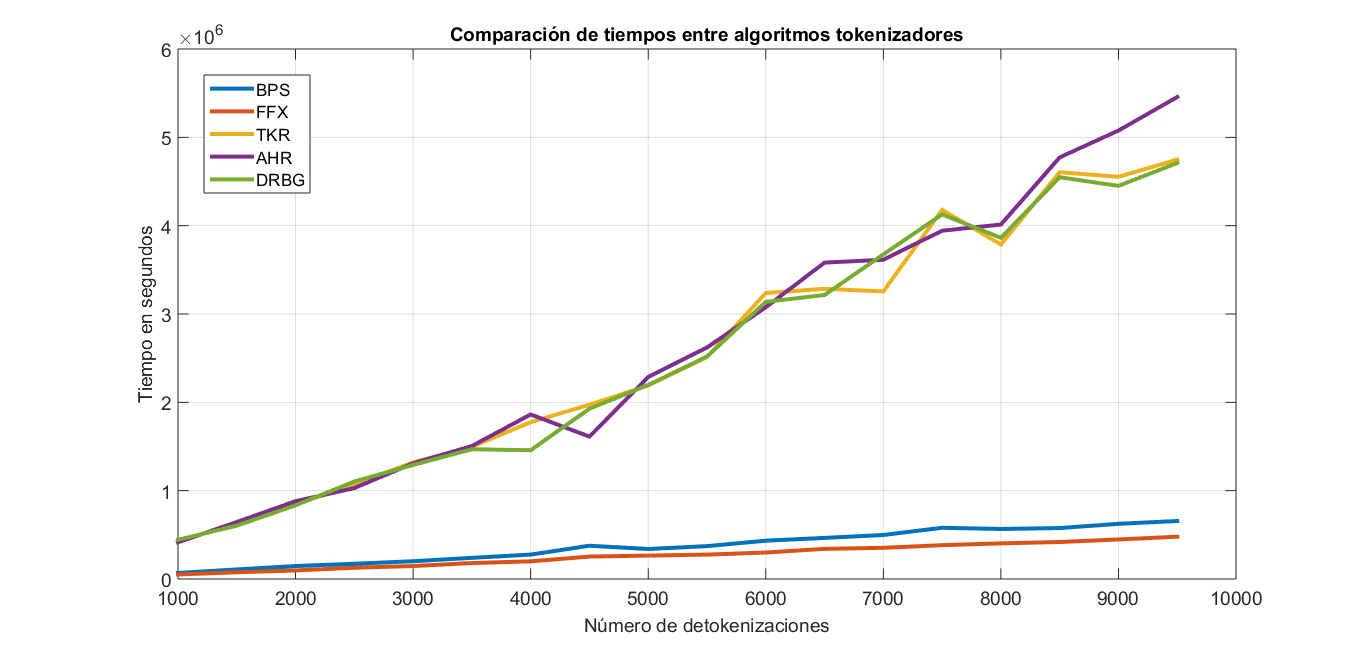
\includegraphics[width=1\linewidth]{diagramas/detok_todos}
      \caption{Tiempos de detokenización.}
    \end{center}
  \end{subfigure}
  \caption{Comparación de tiempos entre algoritmos tokenizadores.}
  \label{figura:tok_todos}
\end{figure}

\begin{figure}
  \centering
  \begin{subfigure}{1\textwidth}
    \begin{center}
      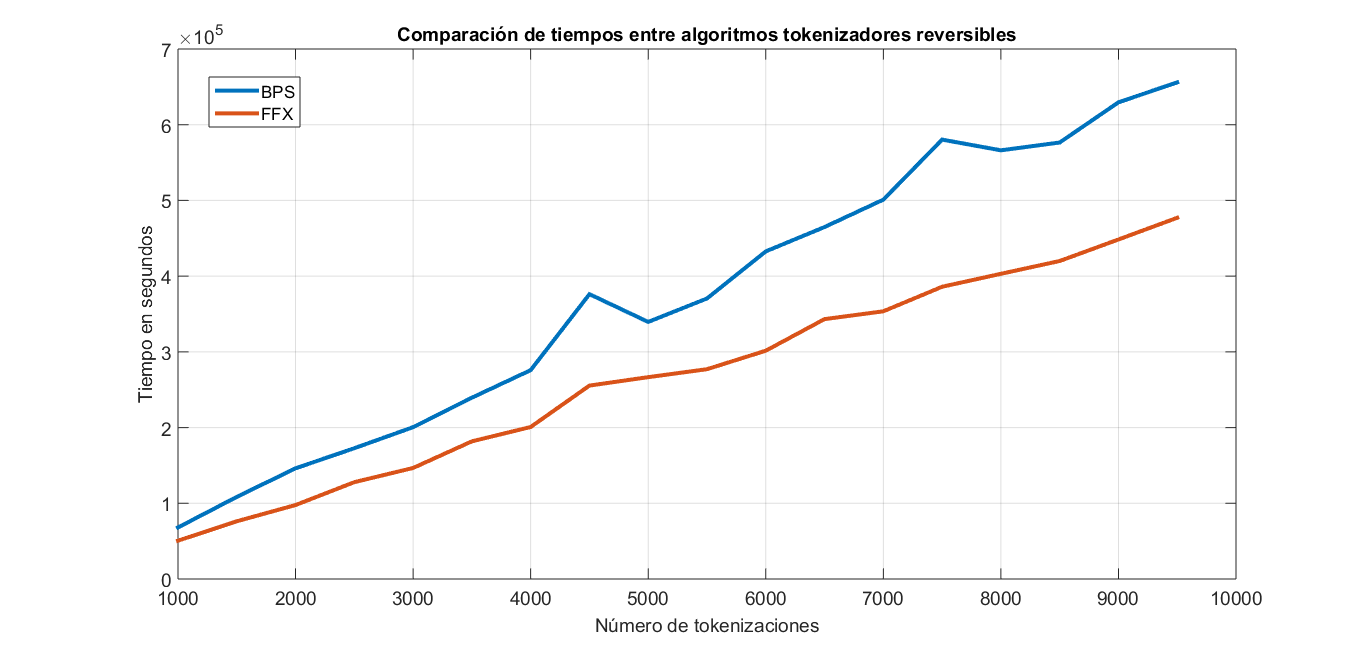
\includegraphics[width=1\linewidth]
        {../../../../../diagramas_comunes/desempenio/tok_rev}
      \caption{Tiempos de tokenización.}
    \end{center}
  \end{subfigure}
  \begin{subfigure}{0.9\textwidth}
    \begin{center}
      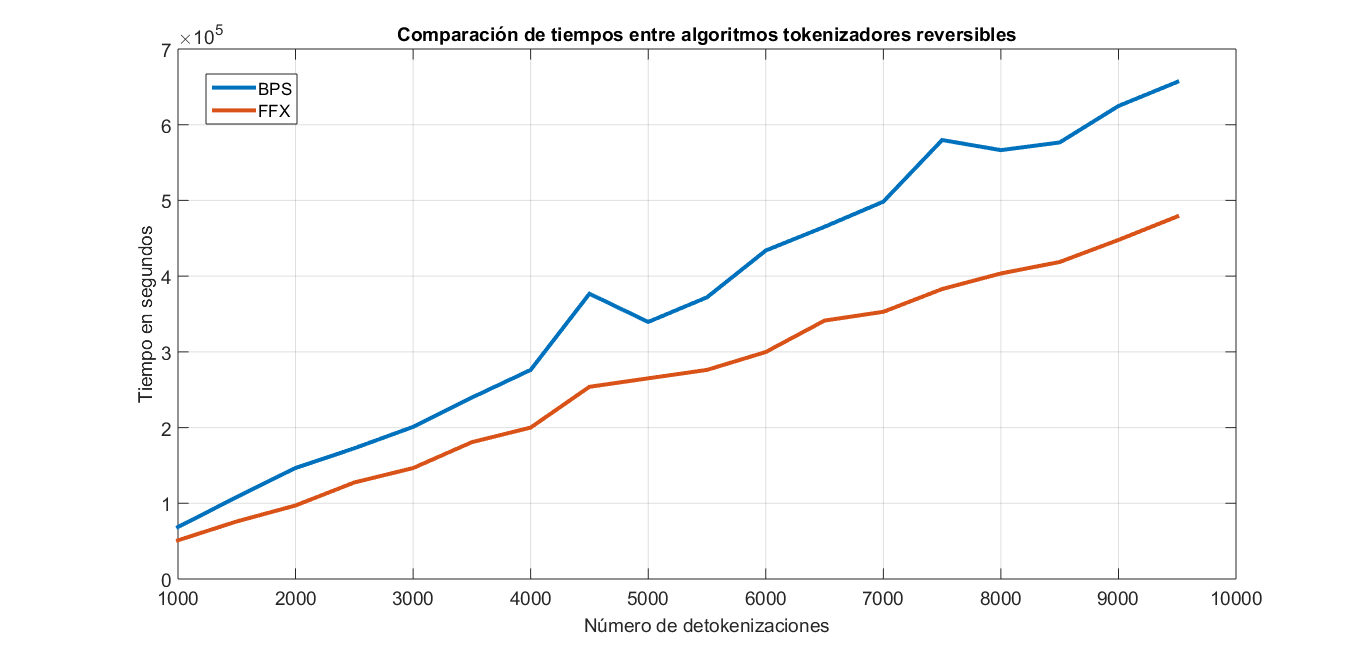
\includegraphics[width=1\linewidth]{diagramas/detok_rev}
      \caption{Tiempos de detokenización.}
    \end{center}
  \end{subfigure}
  \caption{Comparación de tiempos entre algoritmos tokenizadores reversibles.}
  \label{figura:tok_rev}
\end{figure}

\begin{figure}
  \centering
  \begin{subfigure}{1\textwidth}
    \begin{center}
      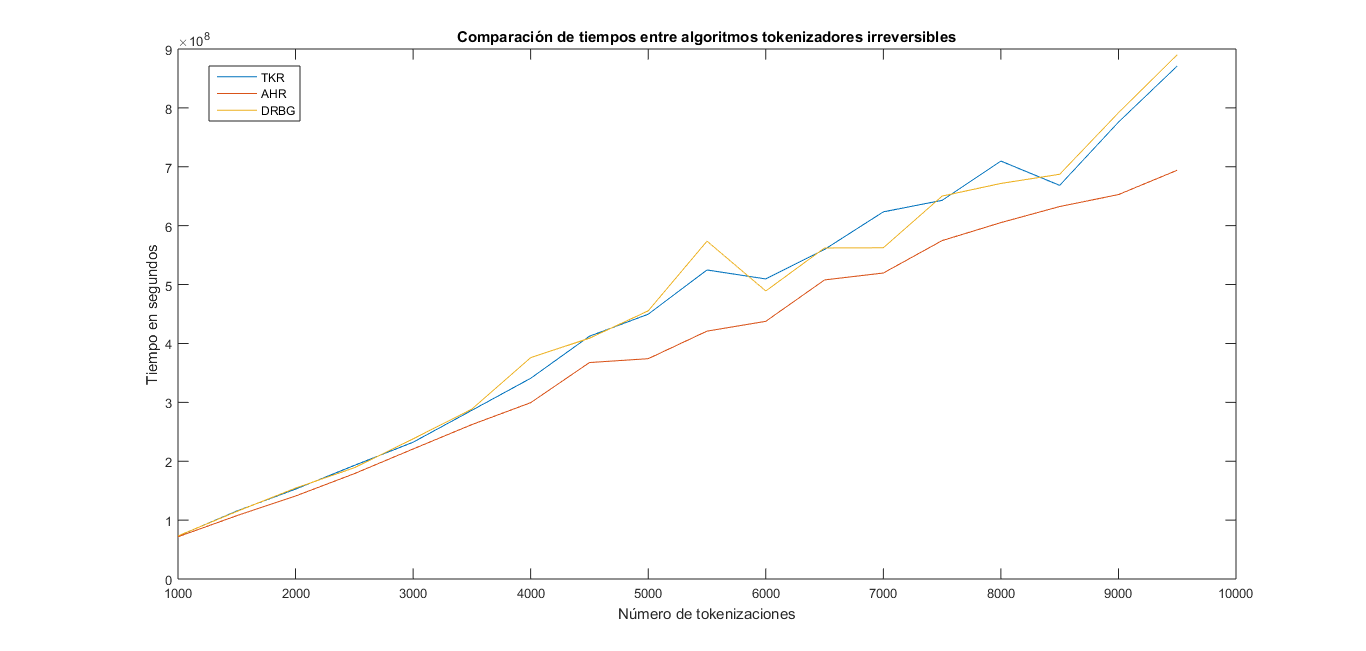
\includegraphics[width=1\linewidth]
        {../../../../../diagramas_comunes/desempenio/tok_irrev}
      \caption{Tiempos de tokenización.}
    \end{center}
  \end{subfigure}
  \begin{subfigure}{0.9\textwidth}
    \begin{center}
      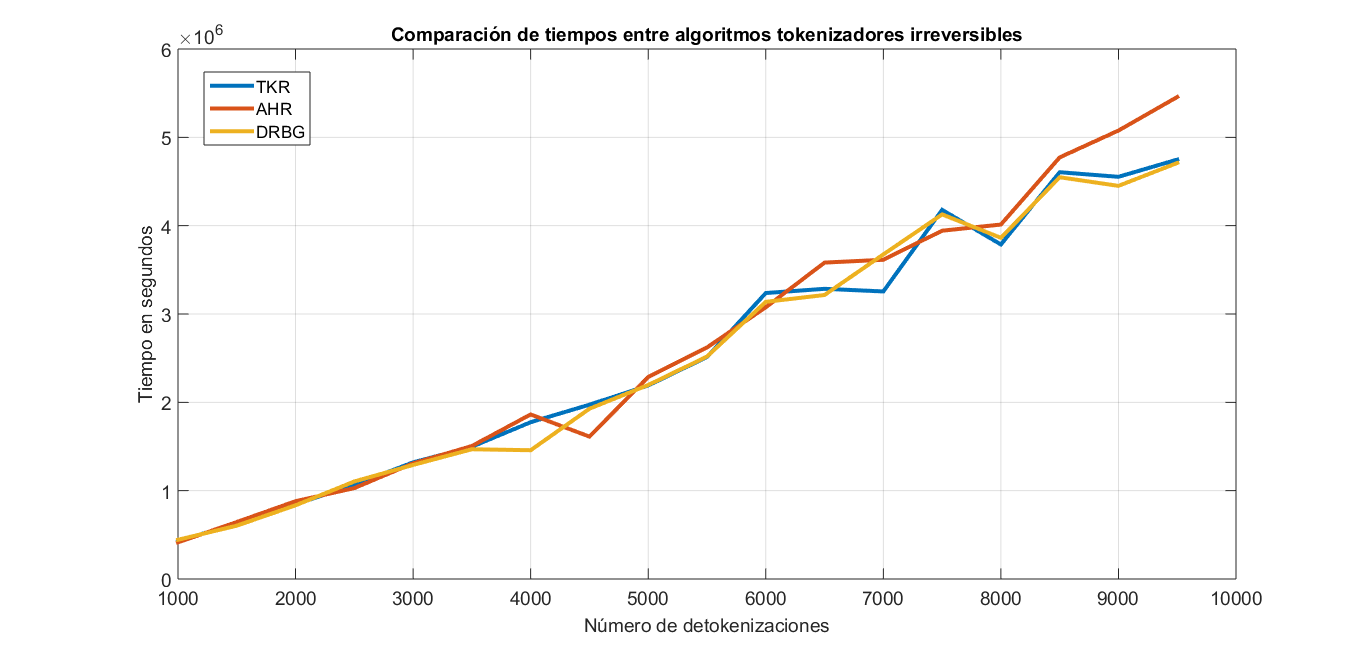
\includegraphics[width=1\linewidth]{diagramas/detok_irrev}
      \caption{Tiempos de detokenización.}
    \end{center}
  \end{subfigure}
  \caption{Comparación de tiempos entre algoritmos tokenizadores irreversibles.}
  \label{figura:tok_irrev}
\end{figure}

\begin{figure}
  \centering
  \begin{subfigure}{1\textwidth}
    \begin{center}
      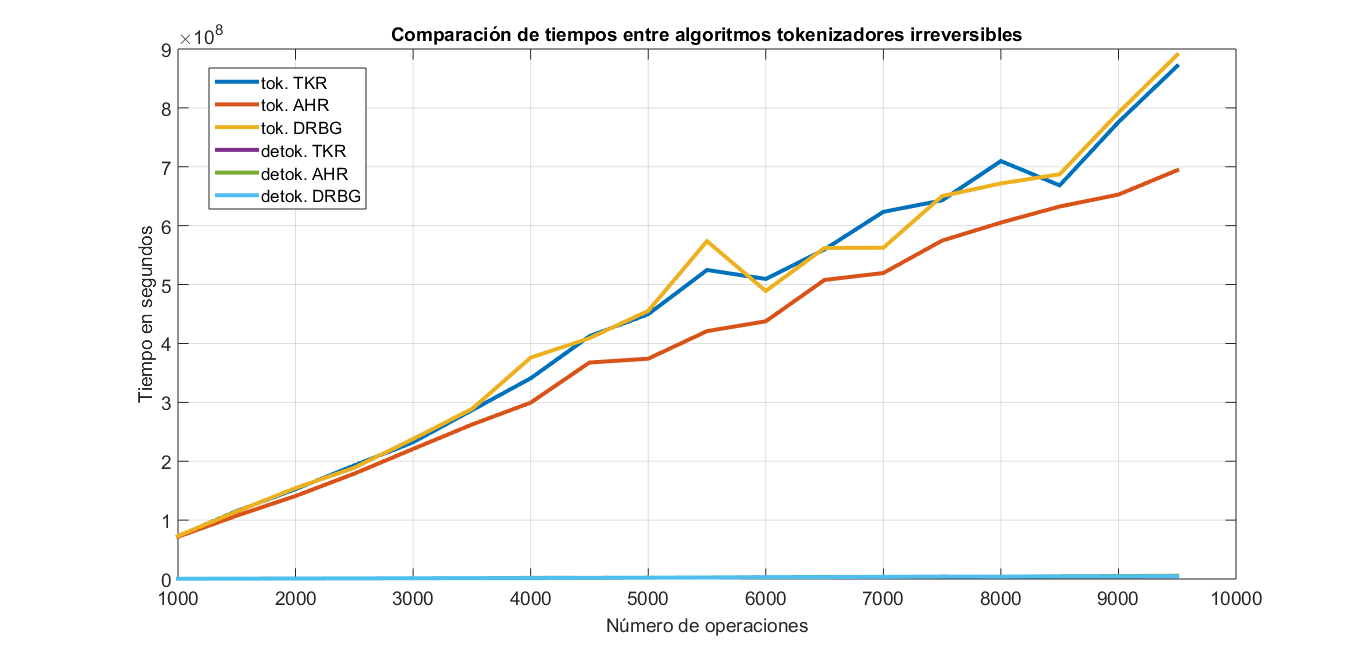
\includegraphics[width=1\linewidth]{diagramas/todo_irrev}
      \caption{Algoritmos de tokenización irreversibles.}
    \end{center}
  \end{subfigure}
  \begin{subfigure}{0.9\textwidth}
    \begin{center}
      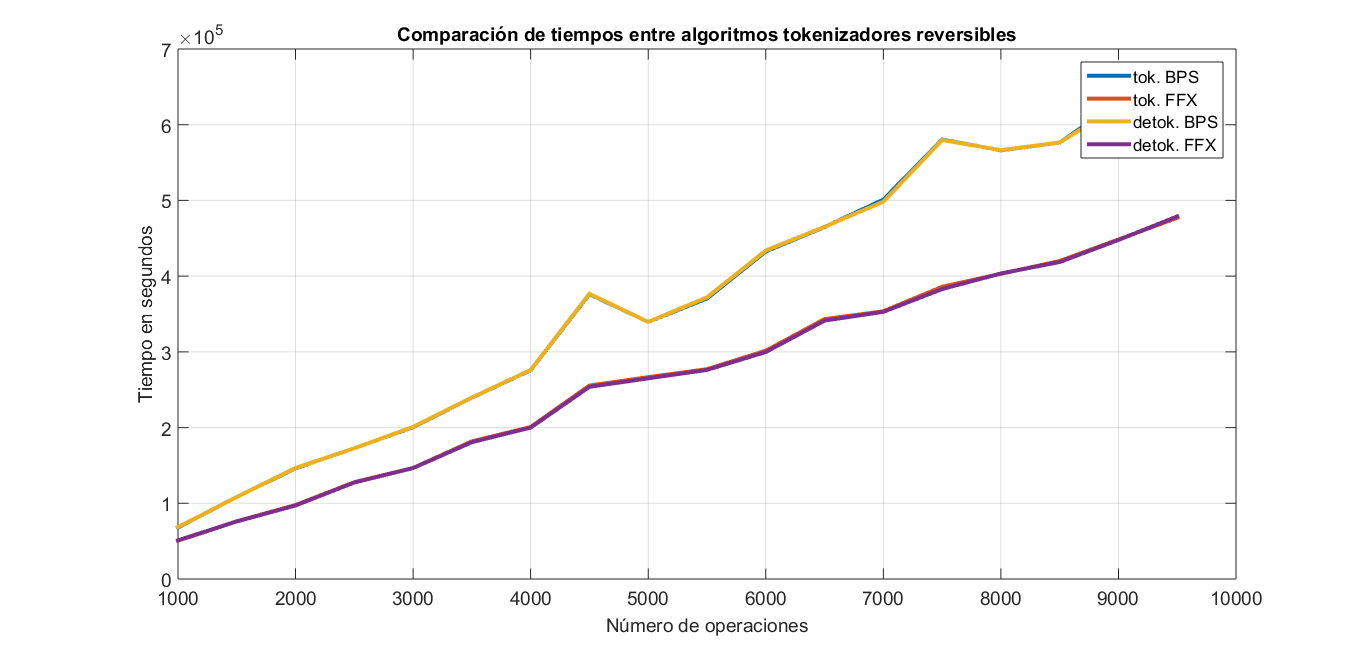
\includegraphics[width=1\linewidth]{diagramas/todo_rev}
      \caption{Algoritmos de tokenización reversibles.}
    \end{center}
  \end{subfigure}
  \caption{Comparación de tiempos de tokenización y detokenización.}
  \label{figura:tok_comp}
\end{figure}
